\documentclass[spanish]{beamer}
\usepackage[ansinew]{inputenc} % Acepta caracteres en castellano
\usepackage[spanish]{babel}    % silabea palabras castellanas
\usepackage{amsmath}
\usepackage{mathtools,cancel} % cancela con una flecha \cancelto{0}{XXXX}
\renewcommand{\CancelColor}{\color{red}} %change cancel color to red
\usepackage{amsfonts}
\usepackage{amssymb}
\usepackage{dsfont}
\usepackage{graphicx}
\usepackage{geometry}
\usetheme{Madrid}
\usecolortheme{beaver}
\usepackage{textpos}
% Logo  en el comienzo 
\addtobeamertemplate{frametitle}{}{%
\begin{textblock*}{100mm}(.85\textwidth,-1cm)
{\includegraphics[height=0.4in, keepaspectratio=true]{/Users/luisnunez/Dropbox/MisDocumentos/UIS/UISImagenInstitucional/UISLOGO.png}}
\end{textblock*}}

\begin{document}

\title{\textbf{Leyes de Kepler} }
\author[L.A. N��ez]{\textbf{Luis A. N��ez}}  
\institute[UIS]{\textit{Escuela de F�sica, Facultad de Ciencias, } \\
\textit{Universidad Industrial de Santander, Santander, Colombia } \\
{\includegraphics[height=0.4in, keepaspectratio=true]{/Users/luisnunez/Dropbox/MisDocumentos/UIS/UISImagenInstitucional/UISLOGO.png}}
}
\date{\today}
\maketitle


\begin{frame}
\frametitle{Agenda}
  \tableofcontents
\end{frame}


%%%%% Diapo 1
\section{Las Leyes de Kepler}
\frame{
  \frametitle{Las Leyes de Kepler}
   \begin{itemize}  
  	\item<1-> {\bf Primera Ley}: los planetas describen �rbitas el�pticas alrededor del Sol, el cual se encuentra en uno de los focos de la elipse. {\bf Forma funcional del potencial gravitacional $V(r)=-\frac{k}{r}$ }.
	\item<2-> {\bf Segunda Ley}: el �rea barrida por unidad tiempo por el radio vector que va desde el Sol al planeta es constante: $\dot{A}=$ cte. {\bf Existencia de un potencial central $V(r)$ y de la conservaci�n de ${\bf L}$}.
	\item<3-> {\bf Tercera Ley}: el cuadrado del per�odo del movimiento es proporcional al cubo del semieje mayor de la �rbita, para todos los planetas: $T_p^2 \propto a^3$. {\bf Forma funcional del potencial gravitacional $V(r)=-\frac{k}{r}$ y conservaci�n de ${\bf L}$ }.
    \end{itemize}
}
%%%%% Diapo 2
\section{Segunda Ley de Kepler}
\frame{
  \frametitle{2da Ley: Velocidad aerolar constante}
   \begin{itemize}  
  	\item<1-> 	Un potencial central $V(r)$ implica la conservaci�n del momento angular $L=\mu r^2 \dot{\theta}=$  constant
  	\begin{figure}[t]
		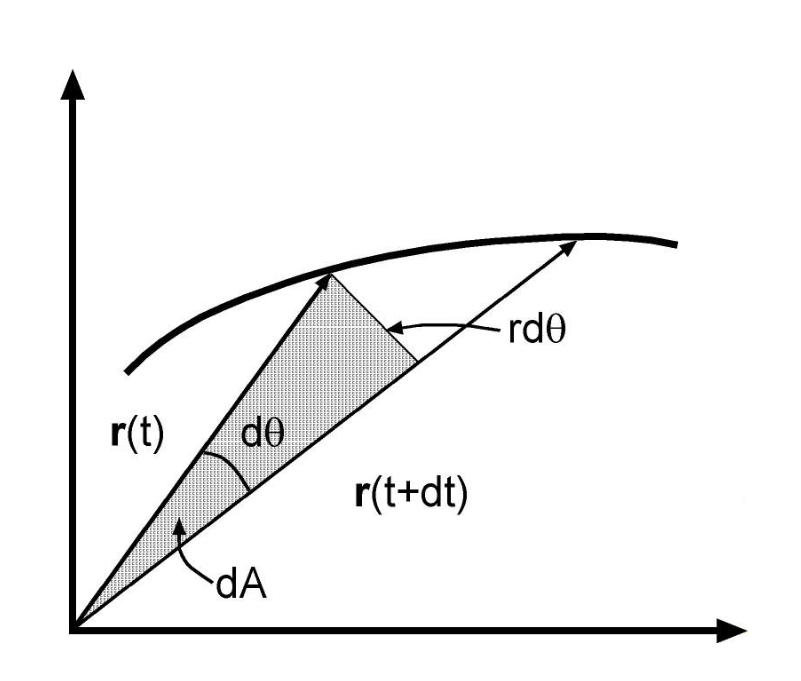
\includegraphics[width=2.0in]{Figuras/VelAerolar.png}
		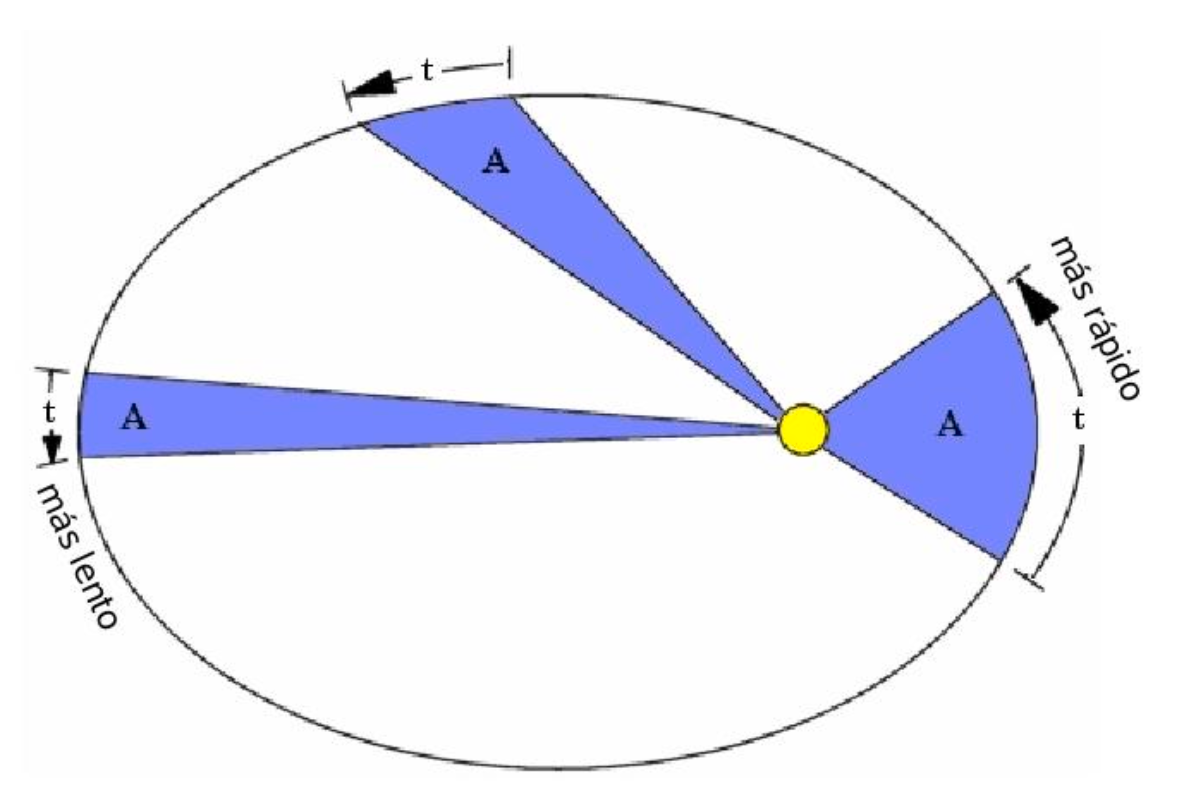
\includegraphics[width=2.0in]{Figuras/VelAerolarKepler.png}
   	\end{figure}
	\item<2-> El diferencial de �rea barrida por el radio vector $\mathbf{r}$ en un tiempo infinitesimal $d t$ es $d A=\frac{1}{2}(r d \theta) r=\frac{1}{2} r^2 d \theta$, entonces $\frac{d A}{d t}=\frac{1}{2} r^2 \frac{d \theta}{d t}=\frac{1}{2} r^2 \dot{\theta}$ es el �rea barrida por unidad de tiempo
	\item<3-> Claramente $\frac{d A}{d t} =\frac{1}{2} r^2\left(\frac{L}{\mu r^2}\right) =\frac{L}{2 \mu}=$ const 
    \end{itemize}
}
%%%%% Diapo 2
\section{Tercera Ley de Kepler}
\frame{
  \frametitle{3ra Ley: $T_p^2 \propto a^3$}
   \begin{itemize}  
  	\item<1-> Si la �rbita es finita, $r \in\left[r_{\min }, r_{\max }\right]$, el �rea total $A$ encerrada por la �rbita barrida por el radio $\mathbf{r}$ en un tiempo igual al per�odo del movimiento $T_p$, es $ A=\frac{l}{2 \mu} \int_0^{T_p} d t=\frac{l}{2 \mu} T_p$
	\item<2-> Si la �rbita es una elipse en el potencial $V(r)=-k / r$, el �rea encerrada elipse $A=\pi a b$, donde $a$, semieje mayor, y $b$ semieje menor 
	\item<3-> Tercera Ley de Kepler en su forma exacta es $T_p=2 \pi \sqrt{\frac{\mu a^3}{k}}$
	\item<4->  $M_S$ es la masa del Sol en el foco, y $m$ del planeta en una �rbita el�ptica. Entonces $m / M_S \ll 1$ y despreciando t�rminos de orden cuadr�tico en $m / M_S$, la masa reducida correspondiente al sistema Sol-planeta se puede expresar como $\mu=\frac{m M_S}{M_S+m}=m\left(1+\frac{m}{M_S}\right)^{-1}=m\left(1-\frac{m}{M_S}+\cdots\right) \approx m$
	\item<5-> Usando $k=G M_S m$ tendremos $T_p^2  \approx \frac{4 \pi^2}{G M_S} a^3 \Rightarrow T_p^2 \propto a^3$

    \end{itemize}
}
\end{document}

%%%%% Diapo 2
\section{Secci�n}
\frame{
  \frametitle{T�tulo transparencia}
   	\begin{itemize}  
  \item<1-> 
    \end{itemize}
}
%%%%% Diapo 2
\section{Secci�n}
\frame{
  \frametitle{T�tulo transparencia}
   	\begin{itemize}  
  \item<1-> 
    \end{itemize}
}
